\documentclass[conference]{IEEEtran}
\IEEEoverridecommandlockouts
% Template version as of 6/27/2024

\usepackage{cite}
\usepackage{amsmath,amssymb,amsfonts}
\usepackage{algorithm}
\usepackage{algorithmic}
\usepackage{graphicx}
\usepackage{textcomp}
\usepackage{xcolor}
\usepackage{booktabs}
\usepackage{url}
\usepackage[hidelinks]{hyperref}
\setlength{\textfloatsep}{6pt plus 1pt minus 2pt}
\setlength{\floatsep}{6pt plus 1pt minus 2pt}
\setlength{\intextsep}{6pt plus 1pt minus 2pt}
\def\BibTeX{{\rm B\kern-.05em{\sc i\kern-.025em b}\kern-.08em
    T\kern-.1667em\lower.7ex\hbox{E}\kern-.125emX}}
\begin{document}

\title{Multi-Sphere SVDD for Vanilla Autoencoder:\\A Process-Control View on Granularity}
\author{\IEEEauthorblockN{Cecil Joseph}
\IEEEauthorblockA{\textit{Department of Applied Mathematics} \\
\textit{Brandenburg University of Technology Cottbus-Senftenberg}\\
Cottbus, Germany \\
0009-0005-2231-139X}
\and 
\IEEEauthorblockN{Martin T. Schorradt}
\IEEEauthorblockA{\textit{Department of Applied Mathematics} \\
\textit{Brandenburg University of Technology Cottbus-Senftenberg}\\
Cottbus, Germany \\
0000-0002-9346-7624}
\and
\IEEEauthorblockN{Michael Breuß}
\IEEEauthorblockA{\textit{Department of Applied Mathematics} \\
\textit{Brandenburg University of Technology Cottbus-Senftenberg}\\
Cottbus, Germany \\
0000-0002-5322-2411}
}

\maketitle

\begin{abstract}
Normal data is rarely one compact cluster. A single Deep Support Vector Data Description sphere is therefore too coarse, while an uncontrolled multi-sphere model can collapse onto one dominant sphere or fragment into many small unstable regions. This paper presents a multi-sphere SVDD pipeline for a vanilla autoencoder with explicit granularity controls: member-count pruning, overloaded-sphere splitting, a hard cap on cluster size, inline center and radius updates, and a chaos factor that biases overflow reassignment away from already saturated spheres. Evaluated on MNIST treated as everything-normal, the controlled pipeline keeps 21 active spheres out of 30 and produces a granular but visually coherent partition: several spheres isolate writing-style variants of the same digit, while mixed spheres pool digits with similar stroke structure. The result is useful as a structural-similarity analysis rather than as a claim of final one-class performance. The same similarity-driven behaviour can also reduce one-class purity when anomalies resemble normal sub-modes. Applying the approach to other datasets is left as future work because preprocessing, backbone choice and stability must be validated carefully.
\end{abstract}

\begin{IEEEkeywords}
Multi-sphere SVDD, vanilla autoencoder, granularity control, prune, split, hard cap, chaos factor, unsupervised clustering, anomaly detection, structure similarity analysis.
\end{IEEEkeywords}

\section{Introduction}
Support Vector Data Description (SVDD) describes normal data by a compact boundary \cite{tax2004support}, in the same spirit as the one-class SVM that estimates the support of a high-dimensional distribution \cite{scholkopf2001estimating}. Deep SVDD replaces the classical kernel representation with a neural encoder and has become a useful one-class learning baseline \cite{ruff2018deep}. In many engineering settings, however, the normal state is not a single compact cloud. A machine can operate in several stable regimes; handwritten digits can appear in several writing styles; simulated engine signals can vary with load, speed and environmental conditions. A single sphere is therefore either forced to grow until it includes all sub-modes (and accepts too much), or it stays small and incorrectly rejects valid but less frequent operating states.

Multi-sphere SVDD addresses this by representing the normal region as a union of \(K\) local spheres \cite{ghafoori2020deep}. In practice, this trades one problem for another. The new question is no longer ``what is the smallest enclosing sphere?'' but ``how many spheres should remain active, how large should they grow, and what happens when one sphere starts dominating the data?''

This paper is an exploratory check of one concrete control approach for this question, not a claim of a method that ``solves'' multi-sphere SVDD. The single phenomenon that the controls actually address is \emph{sphere collapse}: without intervention, one head typically accumulates most of the training mass. In our full-MNIST run this is the iteration-0 reading of Table~\ref{tab:massflow} (\(\sim\!36\)k of \(56\)k training points on a single head). Adding a hard cap on cluster fraction, an overload-driven splitter and a chaos-weighted reassignment of overflow samples brings this dominant fraction back under the cap within a few iterations. In that narrow sense, collapse is controllable; we report it as such.

Two other behaviours commonly attributed to multi-sphere training, \emph{excessive fragmentation} into many small spheres and \emph{non-pure} (mixed) clusters that pool visually related classes, were \textbf{observed in this study as side effects} of fixing collapse rather than as failure modes the loop prevents. Splitting an overloaded sphere with a k-means bisection creates new heads by construction; routing overflow samples with the chaos factor spreads them across the active set; both steps increase the number of active spheres and dilute their class purity. We therefore do \emph{not} claim to suppress fragmentation or to deliver clean class clusters. We claim only that the controls keep collapse bounded, and we report what the resulting partition looks like, read as a structural-similarity decomposition (Section~\ref{sec:struct}).

Two splitting paths are used in the implementation: an overload-driven split inside the rebalancing pass (Section~\ref{sec:control}, C2) and an inline per-epoch split with a concentration-based trigger (Section~\ref{sec:control}, C7). Both feed into the same active-mask update; only the trigger criterion differs.

MNIST is used as a transparent benchmark because the true class labels make cluster purity easy to inspect after training. The broader motivation is engineering data with several normal sub-modes, but this paper does not claim transfer to other datasets. Such transfer requires careful preprocessing, feature design and stability testing, and is therefore treated as future work.

The main contributions, framed accordingly, are:
\begin{enumerate}
    \item An exploratory pipeline for unsupervised multi-sphere SVDD with explicit prune, split and cap operations, and a documented per-epoch split criterion that can be either inverse-distance or silhouette-based.
    \item A chaos factor that softens the hard-cap reassignment and gives an explicit knob between strict and exploratory routing of overflow samples.
    \item A granularity analysis on MNIST that reports what the controlled pipeline actually does: collapse is bounded, fragmentation and mixed-cluster purity are side effects of the same loop, and the upstream knobs that would have to change to attack those side effects directly are the encoder backbone and the embedding geometry.
\end{enumerate}

\section{Materials and Method}

\subsection{Dataset and Preprocessing}
We use the processed MNIST dataset (\(28\times 28\) grayscale, ten classes) with a standard \(80/20\) train/test split. The same label-free preprocessing is used everywhere: global contrast normalization \cite{coates2011analysis} with \(\ell_{1}\) scale, followed by a single linear rescale to \([0,1]\) using one pair \((v_{\min},v_{\max})\) shared across all classes. Class identities never enter the loss; they are only used \emph{after} training, to inspect cluster purity. For the one-class boundary experiment of Section~\ref{sec:occ} the training set is restricted to digit~0; for the structure-discovery experiment of Section~\ref{sec:full} all ten digits are used without labels.

\subsection{Encoder, Heads and Sphere Geometry}
The shared backbone is a vanilla LeNet-style autoencoder \cite{ruff2018deep}. The encoder maps an input image to a 32-d representation; the decoder reconstructs the input. The reconstruction path is essential because it prevents the encoder from mapping every input to the same trivial point, which is the standard Deep SVDD collapse \cite{hojjati2024dasvdd}. The choice of a vanilla backbone is deliberate: it lets the rest of the paper attribute the observed clustering behaviour to the control loop rather than to a specific deep architecture. The cost of this choice is discussed in Section~\ref{sec:limits}: a shallow autoencoder produces a representation that organises samples primarily by visual structural similarity, which is exactly the behaviour we want to highlight here but also a limiting factor for one-class purity.

On top of the encoder we stack \(K=30\) linear projection heads of width \(z=16\). Head \(k\) produces a candidate embedding \(z_{k}=W_{k}\,\mathrm{rep}(x)\). The model maintains a center \(c_{k}\) and radius \(R_{k}\ge 0\) per head. The paper abstracts the geometry through a squared distance value \(D_{k}(x)=\mathrm{dist}^{2}(z_{k},c_{k})\). This is intentional: the contribution is the control loop acting on distances, assignments, centers and radii, not the choice of a particular embedding geometry.

\subsection{Training Pipeline}
The paper reports the method as an engineering pipeline, not as a comparison of source-code variants. The procedure is shown in Algorithm~\ref{alg:pipeline}. It starts with a reconstruction-only warm-up so that the encoder preserves input structure. After warm-up, the nearest active sphere receives the SVDD loss, radii are updated from in-cluster distance quantiles, and the control loop repeatedly prunes weak spheres, splits overloaded spheres, applies the hard cap, and reassigns overflow samples with the chaos factor.

\begin{algorithm}[t]
\caption{Controlled multi-sphere SVDD training.}
\label{alg:pipeline}
\begin{algorithmic}[1]
\REQUIRE training set \(\{x_i\}_{i=1}^{N}\); heads \(K\); cap \(\mathrm{cap}=\lceil\rho_{\max}N\rceil\); thresholds \(\tau_{\min},s_{\min},\rho_{\max}\); chaos factor \(\eta\); overlap margin \(\delta\); soft-boundary \(\nu\); warm-up epochs \(E_{\mathrm{wu}}\); max rebalancing passes \(T\).
\STATE Initialise autoencoder, \(K\) projection heads, centers \(c_k\), active set \(\mathcal{A}=\{1,\dots,K\}\).
\STATE \textbf{Stage 1 (warm-up).} For \(E_{\mathrm{wu}}\) epochs, train encoder-decoder on \(\mathcal{L}_{\mathrm{rec}}\) only; set each \(R_k\) to the \((1-\nu)\)-quantile of in-cluster distances after the last warm-up epoch.
\STATE \textbf{Stage 2 (controlled training).}
\FOR{each training epoch}
    \FOR{each mini-batch}
        \STATE Encode \(x\), compute \(D_k(x)\) for \(k\in\mathcal{A}\) and \(k^{\star}(x)\!=\!\arg\min_{k\in\mathcal{A}}D_k(x)\).
        \STATE Step on \(\mathcal{L}=\mathcal{L}_{\mathrm{rec}}+\lambda_{\mathrm{SVDD}}\mathcal{L}_{\mathrm{SVDD}}+\lambda_{\mathrm{ov}}\mathcal{L}_{\mathrm{ov}}\) (Eqs.~\ref{eq:total}--\ref{eq:overlap}).
    \ENDFOR
    \STATE Recompute centers \(c_k\) and radii \(R_k\) from current assignments (C5).
    \STATE (every \(E_{\mathrm{split}}\) epochs) \textbf{Inline split} via concentration trigger (Eq.~\ref{eq:concentration}) or silhouette-adaptive criterion (C7).
    \STATE \(\mathcal{A}^{\mathrm{prev}}\leftarrow\mathcal{A}\).
    \FOR{\(t=1\) to \(T\)}
        \STATE \textbf{Prune} \(k\in\mathcal{A}\) with \(n_k<\tau_{\min}\) or silhouette \(<s_{\min}\) (C1).
        \STATE \textbf{Split} every overloaded \(k\) with \(n_k>\mathrm{cap}\) by recursive k-means bisection into spare heads (C2).
        \STATE \textbf{Hard cap.} Keep the \(\mathrm{cap}\) nearest points per sphere (C3).
        \STATE \textbf{Reassign overflow} \(x_i\) to \(\arg\min_{k\in\mathcal{A}}\tilde{D}(x_i,k)\) (Eq.~\ref{eq:chaos}) (C4).
        \STATE Shrink source radii via Eq.~\ref{eq:radshrink}.
        \IF{\(\mathcal{A}=\mathcal{A}^{\mathrm{prev}}\)}
            \STATE \textbf{break}
        \ENDIF
        \STATE \(\mathcal{A}^{\mathrm{prev}}\leftarrow\mathcal{A}\).
    \ENDFOR
\ENDFOR
\STATE \textbf{Inference.} Score each test sample with the union margin \(S(x)\) (Eq.~\ref{eq:union}); declare normal if \(S(x)\le 0\).
\end{algorithmic}
\end{algorithm}

\subsection{Training Loss}
\label{sec:loss}
Training has two stages. \textbf{Stage 1} fits the autoencoder with reconstruction loss
\(\mathcal{L}_{\mathrm{rec}}=\mathbb{E}_{x}\|x-\hat{x}\|_{2}^{2}\) only. \textbf{Stage 2} keeps the reconstruction term and adds the multi-sphere SVDD terms,
\begin{equation}
\mathcal{L} \;=\; \mathcal{L}_{\mathrm{rec}} \;+\; \lambda_{\mathrm{SVDD}}\,\mathcal{L}_{\mathrm{SVDD}} \;+\; \lambda_{\mathrm{ov}}\,\mathcal{L}_{\mathrm{ov}},
\label{eq:total}
\end{equation}
with \(\lambda_{\mathrm{SVDD}}=5\times 10^{-5}\) and \(\lambda_{\mathrm{ov}}=10^{-2}\). The SVDD term is the soft-boundary loss applied only to the \emph{nearest} active sphere:
\begin{equation}
\mathcal{L}_{\mathrm{SVDD}} \;=\; \mathbb{E}_{x}\Bigl[R_{k^{\star}}^{2}+\tfrac{1}{\nu}\bigl(D_{k^{\star}}(x)-R_{k^{\star}}^{2}\bigr)_{+}\Bigr],
\label{eq:softboundary}
\end{equation}
where \(k^{\star}(x)\!=\!\arg\min_{k\in\mathcal{A}}D_{k}(x)\), \(\mathcal{A}\) is the active sphere set and \(\nu=0.1\). The radii \(\{R_{k}\}\) are updated after a 5-epoch warm-up as the in-cluster \((1-\nu)\)-quantile of distances. An overlap penalty discourages two active spheres from learning almost the same region,
\begin{equation}
\mathcal{L}_{\mathrm{ov}} \;=\; \frac{1}{\binom{|\mathcal{A}|}{2}}\sum_{\{a,b\}\subset\mathcal{A},\,a<b}\bigl(R_{a}+R_{b}+\delta-\mathrm{dist}(c_{a},c_{b})\bigr)_{+},
\label{eq:overlap}
\end{equation}
with margin \(\delta=0.05\). In practical terms, the penalty is active only when two sphere boundaries are too close or overlap: if the center distance is smaller than the sum of their radii plus the margin, the pair receives a positive cost; otherwise the cost is zero. This keeps the heads from becoming duplicates and leaves room for different spheres to represent different sub-modes. A note on the normalization: dividing by \(\binom{|\mathcal{A}|}{2}\) averages over \emph{all} pairs, including the (typically many) non-overlapping ones whose cost is zero. When \(|\mathcal{A}|\) is large this can shrink the effective gradient of \(\mathcal{L}_{\mathrm{ov}}\) and make the overlap term feel weak in practice. A common workaround is to normalize only by the number of pairs that are actually overlapping, i.e.\ by \(|\{(a,b):\,R_a+R_b+\delta>\mathrm{dist}(c_a,c_b)\}|\) (clipped to be at least \(1\)); this keeps the per-step gradient on the active pairs roughly constant as the active set grows. We use the all-pairs form because \(|\mathcal{A}|\le 30\) here, but the alternative is the more robust choice for larger \(K\). The anomaly score at inference time is the union margin
\begin{equation}
S(x) \;=\; \min_{k\in\mathcal{A}}\bigl(D_{k}(x)-R_{k}^{2}\bigr).
\label{eq:union}
\end{equation}
A point is considered inside the learned normal region if \(S(x)\le 0\), i.e.\ if it lies inside at least one active sphere.

\subsection{Control Mechanisms}
\label{sec:control}
The control mechanisms are the main subject of this paper. They are organised as a small loop that is re-applied during training; each pass can change the active sphere set \(\mathcal{A}\) and recompute centers and radii. Each control is introduced below with the parameter that exposes it, its meaning, and the range of values it can take.

\textbf{(C1) Prune weak spheres.} A sphere \(k\) is removed from \(\mathcal{A}\) if it owns fewer than \(\tau_{\min}\) training samples (any positive integer; we use \(50\)), or if its average silhouette score \cite{rousseeuw1987silhouettes} in the assignment space is below an optional threshold \(s_{\min}\!\in\![-1,1]\) (off in the reported runs). Pruning is the simplest form of granularity control: it removes regions that the model could not justify with data. If everything is pruned, the largest cluster is forcibly kept.

\textbf{(C2) Split overloaded spheres.} An active sphere is overloaded if it owns more than a fraction \(\rho_{\max}\!\in\!(0,1)\) of the training mass (\(\rho_{\max}\!=\!0.20\) here). Overloaded spheres are split by recursive k-means bisection \cite{steinbach2000comparison} into at most a few sub-spheres per call (we allow up to 4): the largest child stays in the original sphere and the smaller children are placed into spare (inactive) heads. The radius of the source sphere is multiplied by a post-split shrink factor in \((0,1]\) (we use \(0.9\)) so the children start with tighter boundaries than the original. Splitting only activates additional capacity where the data actually demands it.

\textbf{(C3) Hard-cap reassignment.} Even after splitting, single batches can push one sphere above the cap \(\mathrm{cap}\!=\!\lceil\rho_{\max}\,N\rceil\). The hard-cap step therefore keeps the closest \(\mathrm{cap}\) points per sphere and reassigns the overflow. Reassignment is greedy: each overflow sample goes to the nearest \emph{non-saturated} active sphere. Hard-cap is the strict component of the control loop and guarantees that no sphere can dominate the data more than \(\rho_{\max}\).

\textbf{(C4) Chaos factor for soft overflow routing.}
The plain hard-cap rule above is deterministic and tends to fill new spheres in a fixed order. To make the overflow routing more flexible without losing the cap, we add a saturation penalty that scales with the chaos factor \(\eta\). For overflow sample \(x_{i}\) and active sphere \(k\), define the saturation \(s_{k}=n_{k}/\mathrm{cap}\), where \(n_{k}\) is the current count assigned to sphere \(k\), and the mean local distance scale
\begin{equation}
\bar{D}_{i} \;=\; \frac{1}{|\mathcal{A}|}\sum_{k\in\mathcal{A}} D_{k}(x_{i}).
\label{eq:meanD}
\end{equation}
The effective routing cost for the overflow step is
\begin{equation}
\tilde{D}(x_{i},k) \;=\; D_{k}(x_{i}) \;+\; \eta\,s_{k}\,\bar{D}_{i},
\label{eq:chaos}
\end{equation}
and the sample is routed to \(\arg\min_{k\in\mathcal{A}}\tilde{D}(x_{i},k)\) instead of to the strictly nearest active sphere. The interpretation is straightforward:
\begin{itemize}
    \item \(\eta = 0\): pure greedy nearest-non-full routing; tends to concentrate overflow into a few neighbouring spheres.
    \item \(\eta\) small (default \(0.15\)): mild penalty against already saturated spheres; encourages a more diverse usage of the active set.
    \item \(\eta\) large: aggressive avoidance of full spheres; can move samples noticeably far from their natural nearest sphere.
\end{itemize}
In engineering terms, \(\eta\) is the knob that decides whether the rebalancing step should follow the strict geometry of the embedding or trade some geometric fidelity for a more even coverage. Cluster radii are also reduced after rebalancing if the source sphere was over the cap,
\begin{equation}
R_{k} \;\leftarrow\; R_{k}\cdot\max\bigl(0.7,\;1-0.3\min(1,\eta+0.2)\bigr),
\label{eq:radshrink}
\end{equation}
so that a more chaotic routing also tightens the source-sphere boundary and the overall structure does not become too loose.

\textbf{(C5) Inline radius and center updates.} The default variant of the pipeline (the one used to produce the figures in this paper) re-fits the radii and the centers \emph{during} training, not only at the end. Every few epochs the centers of active spheres are recomputed from their current assignments, and the radii are updated as the \((1-\nu)\)-quantile of in-cluster distances. This inline update is what makes the active mask responsive: a sphere that loses members during one epoch can be pruned in the next; a sphere that gains many members can be split.

\textbf{(C6) Iterative rebalancing loop.} Steps C1--C3 are wrapped in an outer loop of up to \(T\) iterations (we use \(T\!=\!4\); any small positive integer works in practice). Each iteration re-evaluates the assignments and decides whether further pruning, splitting or capping is needed. The loop terminates early when no control step changes the active mask. In the reported MNIST run the loop converges within four iterations, with the dominant sphere shrinking from \(\sim\!36\,\mathrm{k}\) to under the cap of \(11\,209\) samples.

\textbf{(C7) Inline split with a concentration trigger.} In parallel with the rebalancing-pass overload split (C2), the trainer runs a per-epoch inline splitter on the current training assignments. The default v2 trigger is the per-cluster concentration score
\begin{equation}
\mathrm{score}(k) \;=\; \mathbb{E}_{i\in k}\!\left[\tfrac{1}{\sqrt{D_{k}(x_{i})+\varepsilon}}\right],
\label{eq:concentration}
\end{equation}
where \(D_{k}(x_{i})\) is the nearest-sphere squared distance and \(\varepsilon\) a small constant; a split fires when \(\mathrm{score}(k)\) exceeds a configurable threshold and the cluster has at least \(\mathrm{min\_members}\) points. In the v3 pipeline used to produce the figures of this paper, the trigger callable is replaced at startup by a silhouette-adaptive variant that fires when sphere \(k\)'s mean silhouette drops below \(0.2\) or its negative-silhouette fraction exceeds \(0.1\); both variants share the same scheduling slot and only the criterion differs. Optional assignment-shaping terms (radius shrinkage at inference, inside penalty, assignment-gap and entropy penalties on cluster ownership) also exist in the trainer but were not enabled in the reported runs.

\subsection{Evaluation}
\textbf{Configurations.} We report two configurations of the pipeline. The \emph{full control loop} -- all of C1--C7 active -- is used for the all-digits structure-discovery experiment (Section~\ref{sec:full}, Table~\ref{tab:massflow}). The \emph{inline-only} configuration -- only the inline center/radius update of C5 and the member-count side of C1 are active; the overload split (C2), hard cap (C3), chaos-weighted reassignment (C4), iterative rebalancing (C6) and inline split trigger (C7) are disabled -- is used for the digit-0 OCC stress test (Section~\ref{sec:occ}, Table~\ref{tab:norm0_auc}). The pair lets us compare the controlled active-set behaviour against an ablation in which only the inline active mask responds during training.

\textbf{Diagnostics.} Two diagnostics are reported. First, a granularity diagnostic on the controlled all-digits run: each test sample is assigned to its nearest active sphere, and the row-normalised \(P(d\mid k)\) and column-normalised \(P(k\mid d)\) are computed from the test labels. These two matrices are complementary engineering views: \(P(d\mid k)\) tells what a learned sphere has captured, \(P(k\mid d)\) tells whether a known class is concentrated in one sphere or scattered across several. We also show t-SNE projections, sample grids per sphere and per-cluster input-space saliency maps of the union margin (Eq.~\ref{eq:union}). Second, an OCC stress test on a digit-0 variant (Section~\ref{sec:occ}) confirms the structural-similarity limitation in classical AUC terms.

\section{Results}

\subsection{Full-MNIST Structure Discovery}
\label{sec:full}
The main experiment is the controlled all-digits baseline: it trains on all ten digits without labels, with the split, hard-cap and hybrid rebalancing controls enabled. This setting is used to study whether the control mechanisms can discover sub-structure when no labels are used during optimization. Starting from 30 candidate spheres, the control loop ends with 21 active spheres on the test analysis (\(N=13{,}955\)). Figure~\ref{fig:hulls} shows the resulting partition. The key observation is not that every sphere maps to one digit, but that the controls produce a useful range of granularities: some spheres become highly pure, others remain deliberately mixed and indicate regions where the model would benefit from finer control. The OCC stress test of Section~\ref{sec:occ} below uses the same encoder and head set with the post-processing controls disabled; it retains 20 of 30 candidate heads, while the full control loop here settles on a similarly balanced 21 of 30 on a harder ten-class task that would otherwise collapse to a single dominant head (cf.\ Table~\ref{tab:massflow}, iteration~0). A multi-seed confirmation is still required.

\begin{figure*}[t]
\centering
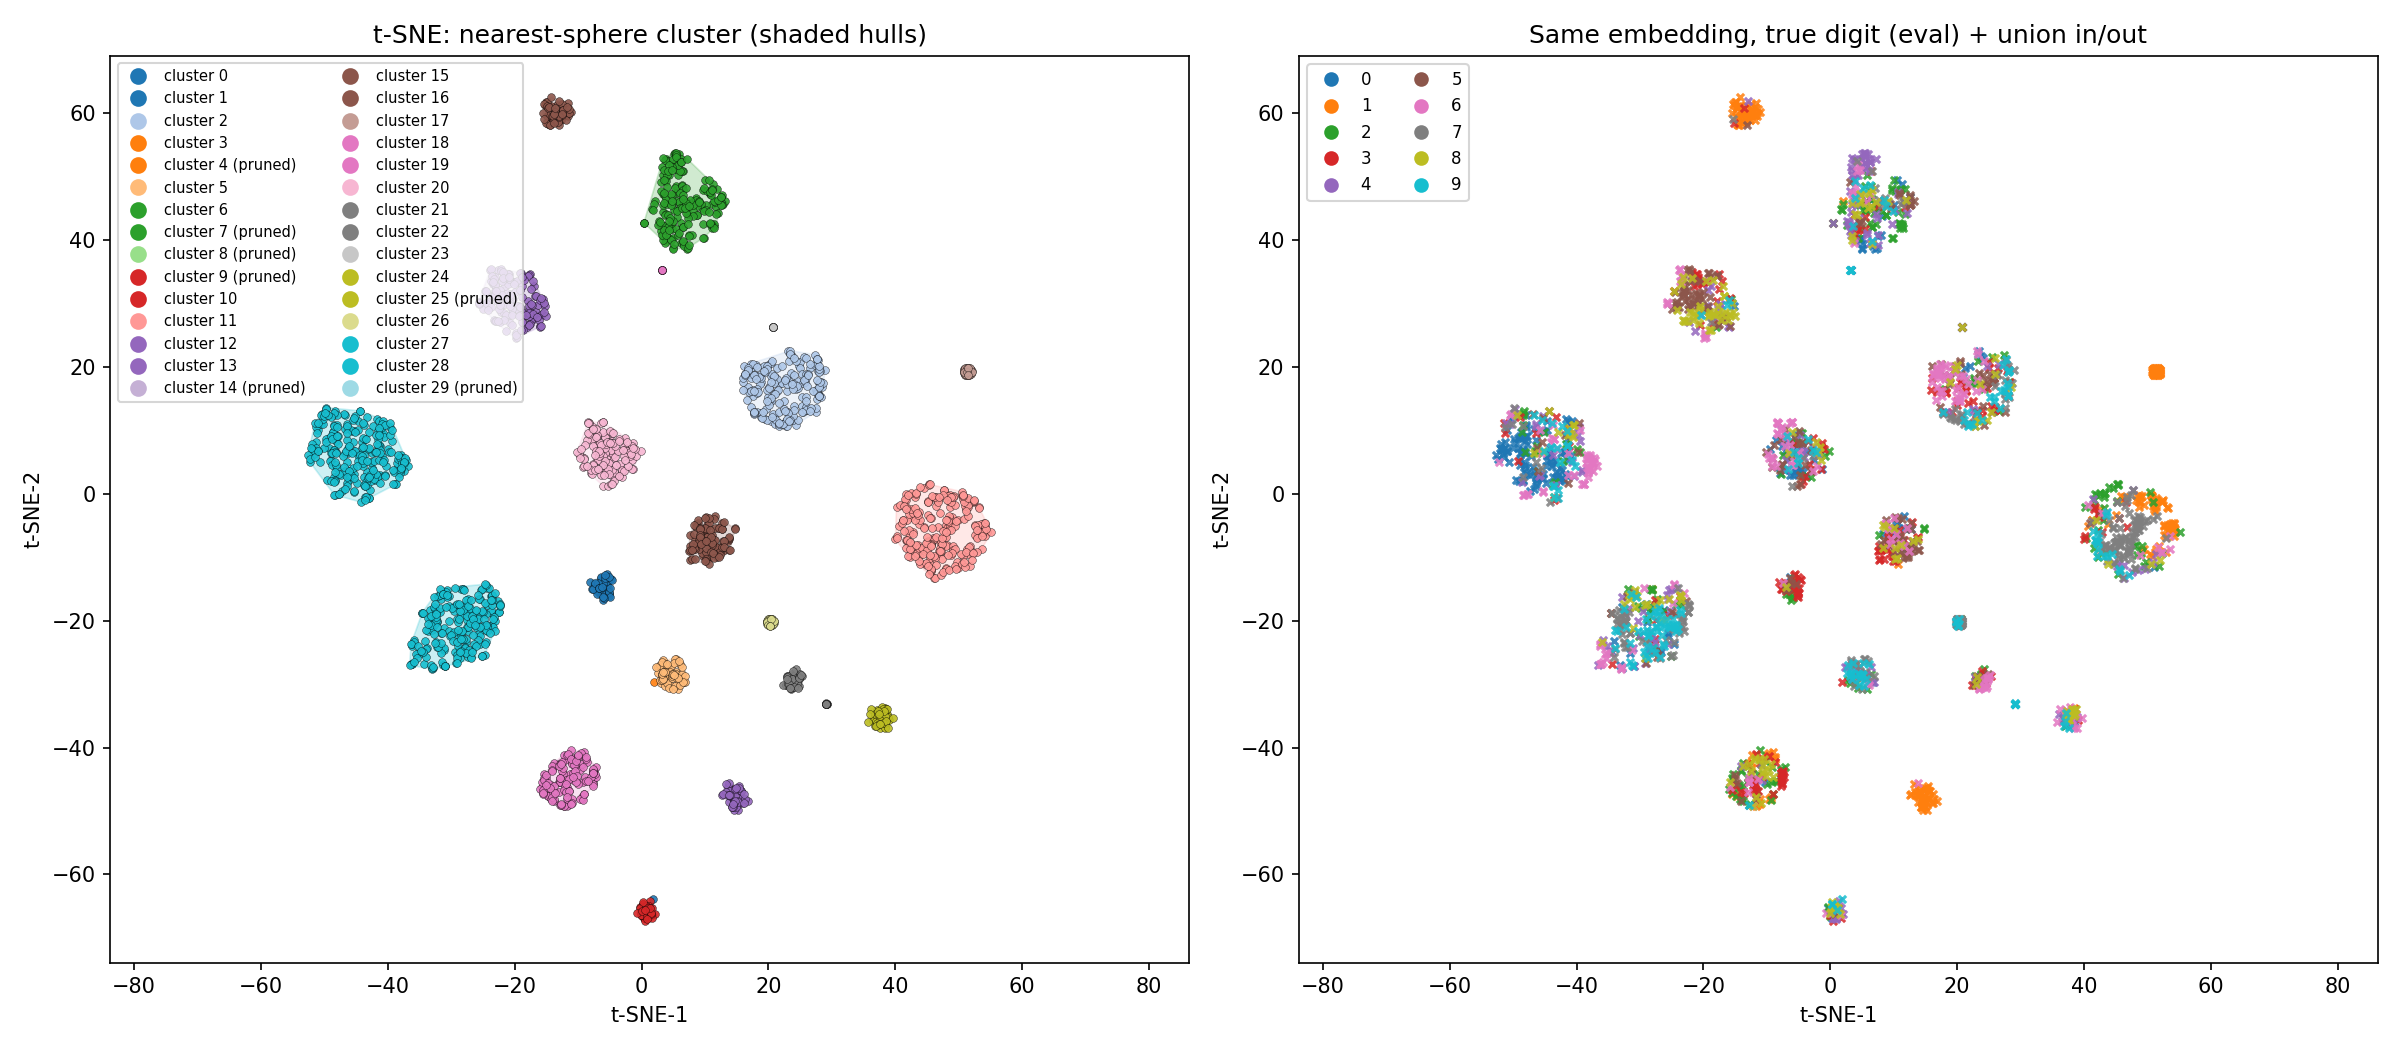
\includegraphics[width=0.95\textwidth]{tsne_unsup_v2_nearest_z.png}
\caption{t-SNE of nearest active-sphere embeddings on the MNIST test split after the control loop. 21 of 30 candidate spheres remain active; pruned heads are marked in the legend.}
\label{fig:hulls}
\end{figure*}

\subsection{Granularity and Structural Similarity}
\label{sec:struct}
The full-MNIST run is set up as an everything-as-normal analysis: no class label is used for training and no class is held out as anomalous. The purpose is to ask what kind of partition the control loop converges to when the model is allowed to discover structure freely. Cluster purity is summarised in Fig.~\ref{fig:heatmaps} and Table~\ref{tab:topclusters}.

Three active spheres are nearly mono-class: sphere~12 with \(99.7\%\) digit~1, sphere~17 with \(96.3\%\) digit~1, and sphere~15 with \(92.9\%\) digit~1. These spheres are not duplicates; visually, they correspond to different writing styles of the same digit (vertical strokes, slanted strokes, strokes with a serif). Several other spheres are clearly class-coherent: sphere~23 is \(64.9\%\) digit~0, sphere~26 is \(69.0\%\) digit~7, sphere~21 is \(76.3\%\) digit~9.

Reading the heatmap in Fig.~\ref{fig:heatmaps} along the rows confirms a consistent pattern: within a cluster the dominant digits are visually related, and within a digit the active spheres correspond to clearly different writing styles. The mixed clusters obey the same rule. Sphere~2 (\(n\!=\!1640\), entropy \(2.13\) nats) pools digits whose strokes share curves and loops -- mainly \(3\), \(5\) and \(6\). Sphere~6 (\(n\!=\!1421\), entropy \(2.02\) nats) groups digits with parallel vertical strokes -- mainly \(2\), \(4\) and \(8\). These spheres are not random mixtures; every class that lands in them is visually compatible with the cluster's structural pattern. We therefore read the partition as a structural-similarity decomposition: clusters are granular and at the same time visually consistent, and the mixed clusters are the unavoidable consequence of doing this without labels.

This view changes how the mixed clusters should be interpreted. They are not failures of the method; they are a diagnostic that says the vanilla LeNet representation cannot pull these classes apart on visual cues alone. A natural follow-up is therefore not only to retighten \(\rho_{\max}\) or relax \(\eta\), but also to revisit the backbone (see Section~\ref{sec:limits}).

\begin{figure*}[t]
\centering
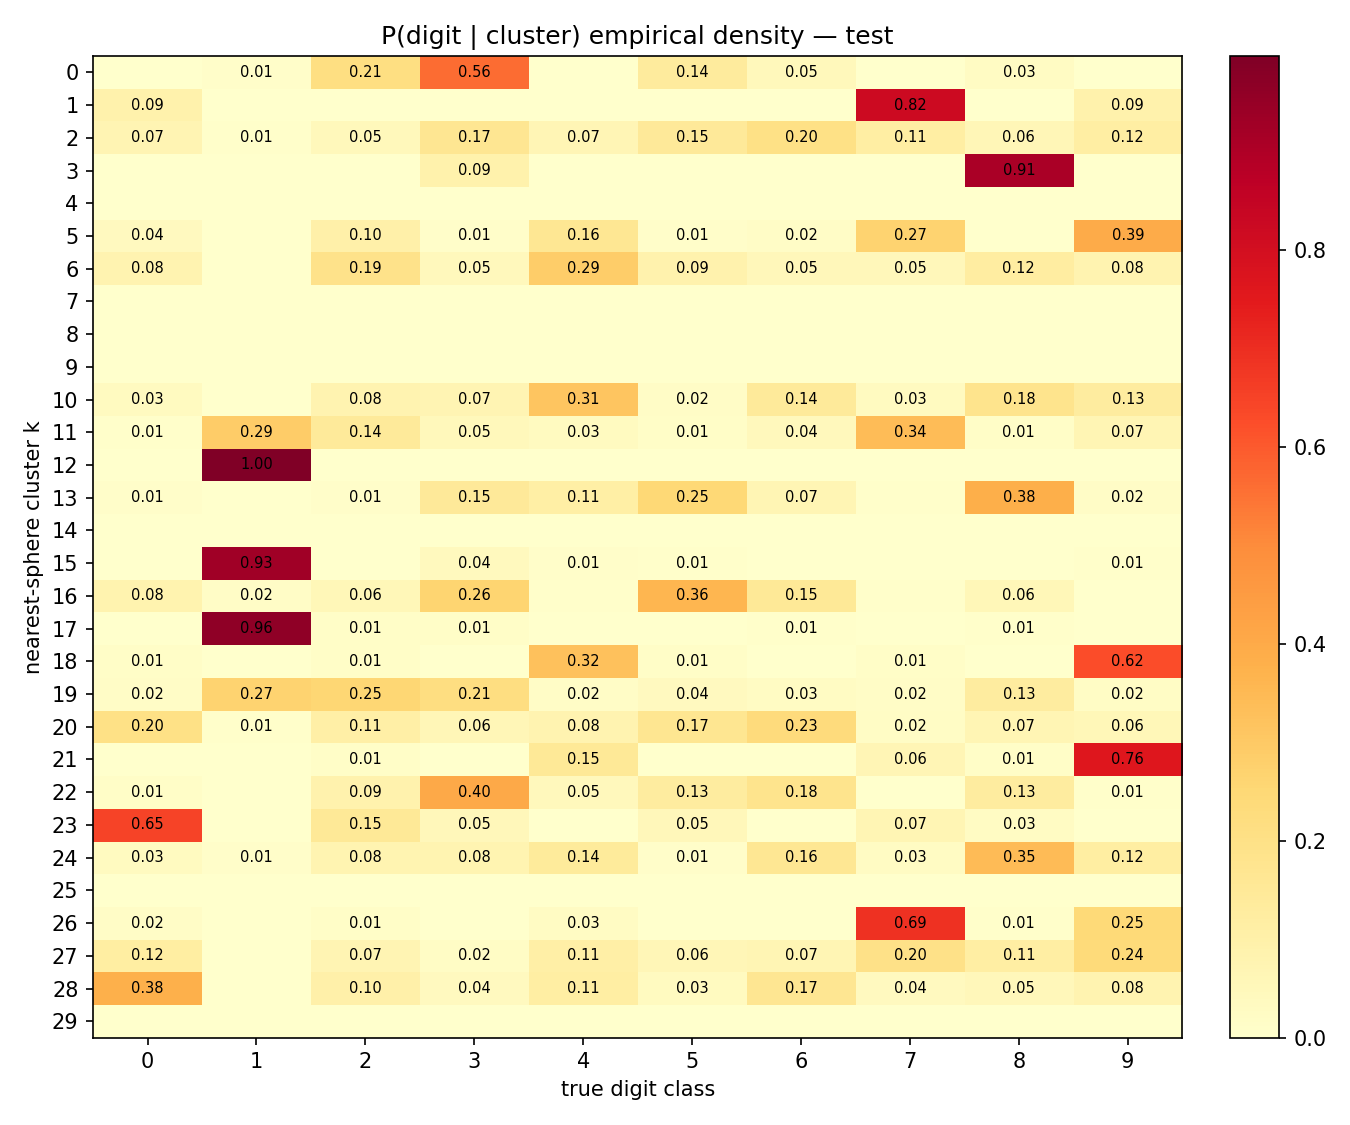
\includegraphics[width=0.85\textwidth]{hotspot_P_digit_given_cluster.png}
\caption{\(P(d\mid k)\): empirical class density inside each active sphere on the MNIST test split. Rows are spheres, columns are true digits; pruned rows are empty.}
\label{fig:heatmaps}
\end{figure*}

\begin{table}[t]
\centering
\caption{Top class-coherent active spheres after the control loop, MNIST test split. Entropy in nats; \(n\) is sphere population.}
\label{tab:topclusters}
\begin{tabular}{rrrcr}
\toprule
\(k\) & \(n\) & dominant digit \(d^{\star}\) & \(P(d^{\star}\mid k)\) & entropy \\
\midrule
12 & 358  & 1 & 0.997 & 0.02 \\
17 & 161  & 1 & 0.963 & 0.21 \\
15 & 364  & 1 & 0.929 & 0.36 \\
3  & 11   & 8 & 0.909 & 0.30 \\
1  & 11   & 7 & 0.818 & 0.60 \\
21 & 80   & 9 & 0.763 & 0.77 \\
26 & 155  & 7 & 0.690 & 0.86 \\
23 & 74   & 0 & 0.649 & 1.16 \\
18 & 77   & 9 & 0.623 & 0.89 \\
0  & 317  & 3 & 0.565 & 1.23 \\
\midrule
2  & 1640 & 6 & 0.201 & 2.13 \\
6  & 1421 & 4 & 0.285 & 2.02 \\
\bottomrule
\end{tabular}
\end{table}

\subsection{Effect of the Control Loop on Sphere Mass}
\label{sec:massflow}
Table~\ref{tab:massflow} traces the size of the largest active sphere across the four iterations of the control loop on the all-digits run. Iteration~1 starts from the autoencoder warm-up and shows the worst case: a single sphere holds \(\sim\!36\)k of the \(56\)k training points, far above the cap of \(11\,209\) (\(\rho_{\max}=0.20\)). Member-count pruning alone leaves this sphere intact. Activating the split rule at iteration~1 redistributes the overload across spare heads, but iteration~2 still shows a near-collapse on a different head. The combination of split, hard cap and chaos-weighted reassignment is what drives the dominant fraction back under the cap by iteration~4.

\begin{table}[t]
\centering
\caption{Largest active sphere across iterations of the control loop (full-MNIST run, \(N=56{,}045\)).}
\label{tab:massflow}
\begin{tabular}{lrrr}
\toprule
iteration & largest sphere \(n\) & cap & active spheres \\
\midrule
0 (init)     & 36{,}293 & 11{,}209 & 30 \\
1 after C1--C3 & 12{,}970 & 11{,}209 & 24 \\
2 after C1--C3 & 12{,}970 (split) & 11{,}209 & 23 \\
3 after C1--C3 & 8{,}767  & 11{,}209 & 25 \\
4 after C1--C3 & 8{,}424  & 11{,}209 & 21 \\
\bottomrule
\end{tabular}
\end{table}

\subsection{Visual Cluster Diagnostics}
Figure~\ref{fig:samples} shows raw MNIST samples drawn from each active sphere. The mono-class digit-1 spheres contain different writing styles, the zero-dominated sphere contains round shapes, and the mixed spheres contain visually related digits rather than random samples -- the same kind of sanity check that confusion matrices provide for supervised models. Figure~\ref{fig:neural} shows mean encoder conv2 activations per cluster, upsampled to input size; they reveal which pixels drive the boundary of each sphere. Similar diagnostics may help on engineering signals but their reliability has not yet been validated there.

\begin{figure}[t]
\centering
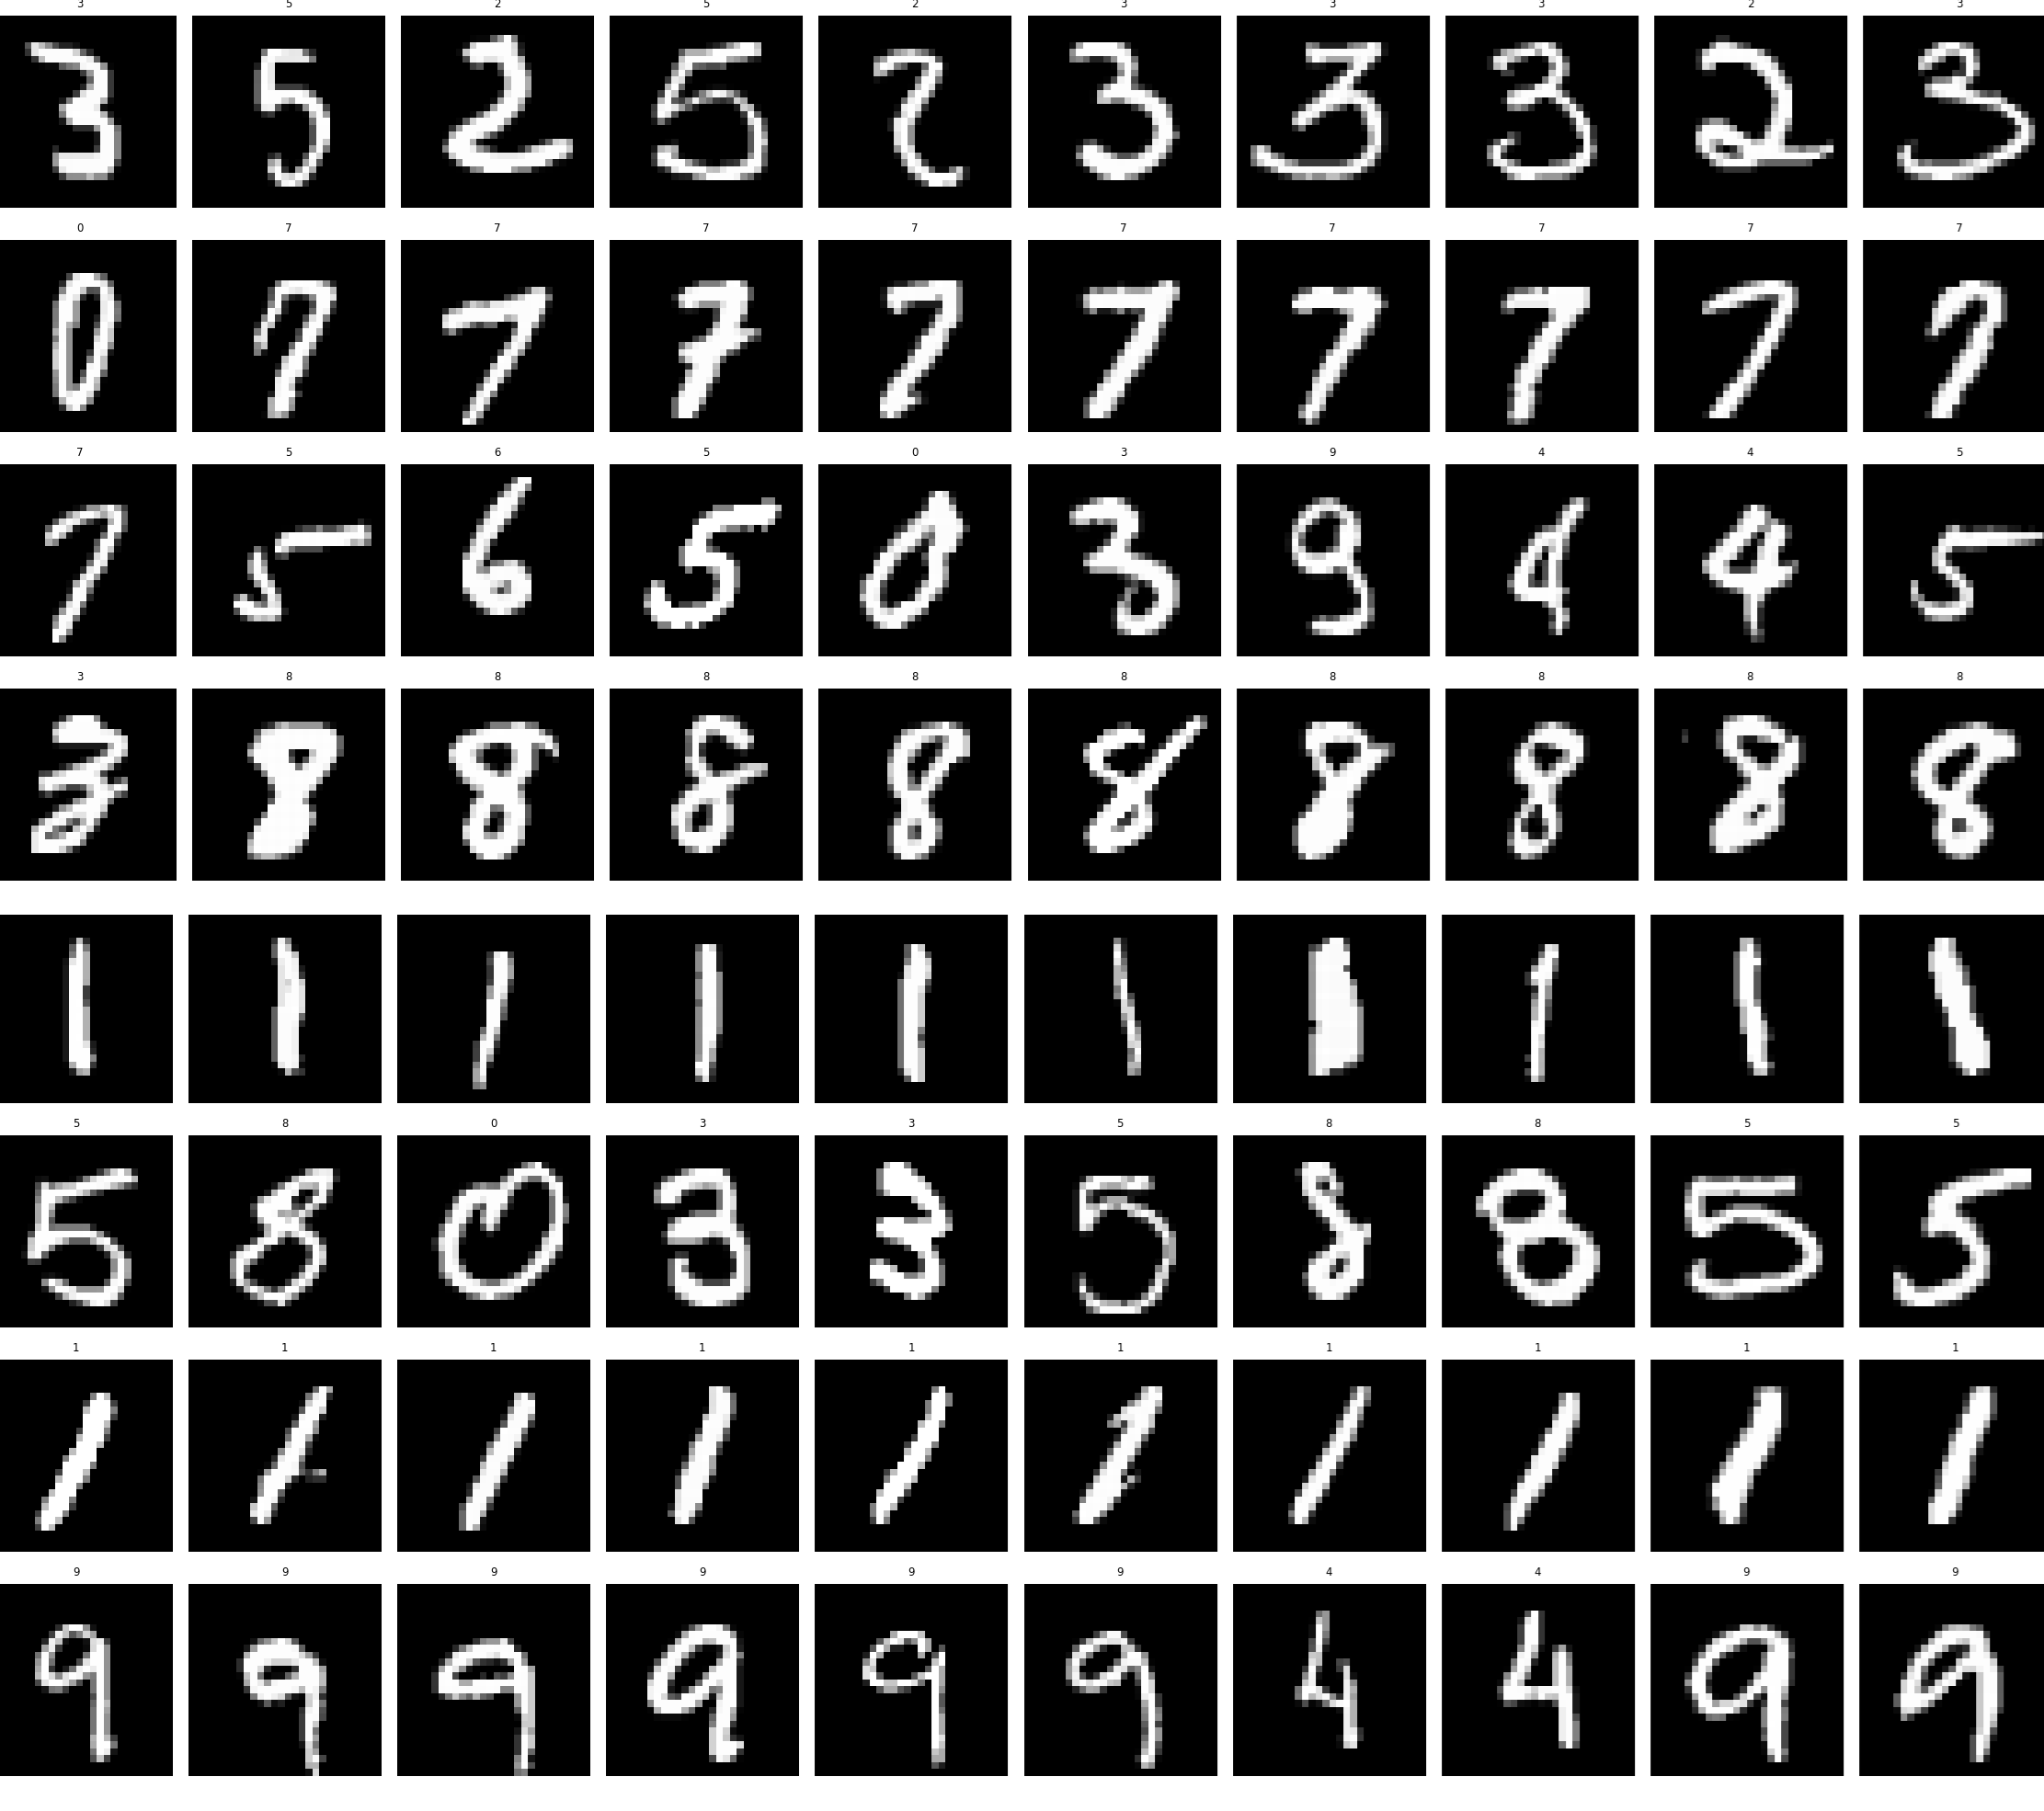
\includegraphics[width=0.55\columnwidth]{SamplesFixed.png}
\caption{Test digits per active cluster spheres}
\label{fig:samples}
\end{figure}

\begin{figure}[t]
\centering
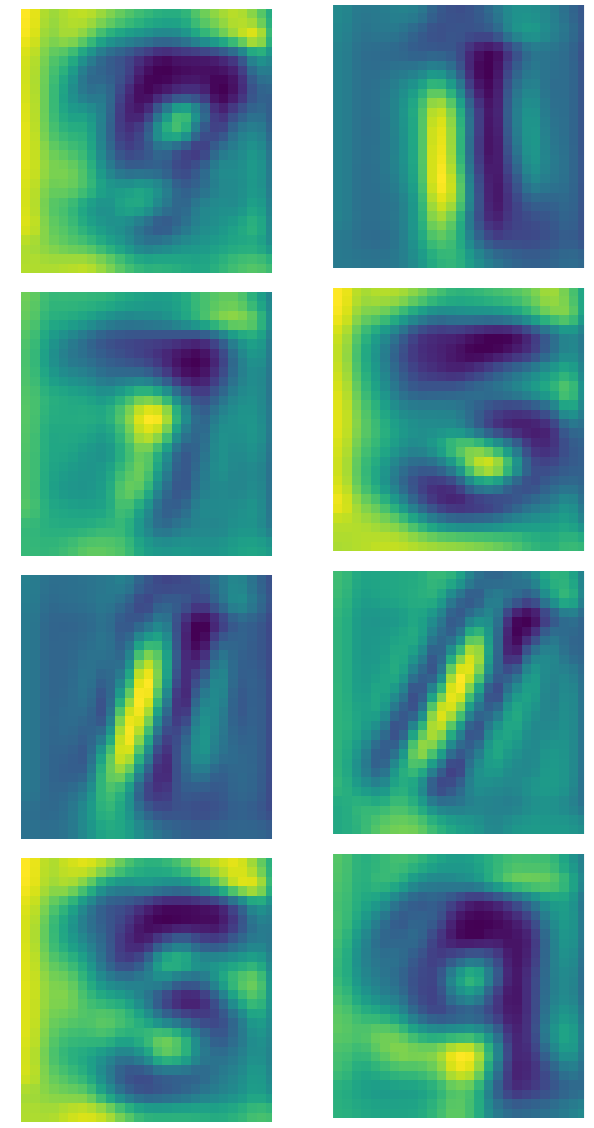
\includegraphics[width=0.25\columnwidth]{NeuralFixed.png}
\caption{Per-cluster neural hotspots. Mean conv2 activation upsampled to input size.}
\label{fig:neural}
\end{figure}

\subsection{One-Class Boundary Test (Stress Test)}
\label{sec:occ}
As a stress test we run the pipeline as a classical one-class detector: digit~0 is the only normal class, and the test set contains all ten digits. Table~\ref{tab:norm0_auc} reports a single-run AUC profile from an inline-only digit-0 configuration (overload split and hybrid rebalancing disabled, only the inline active mask is updated). These numbers are initial observations, not a stability claim; a deeper multi-seed study is still required. Digit~0 itself is scored well (\(0.940\)) but the macro AUC stays near chance (\(0.504\)); several non-zero digits are routed \emph{into} the union more confidently than the held-out digit~0, showing that the boundary follows stroke similarity rather than semantic class identity. The inline active mask keeps \(20\) of \(30\) candidate spheres -- digit~0 is decomposed into many writing-style sub-modes rather than wrapped by a single ball -- so the boundary favours \emph{granularity over purity}. The same structural-similarity effect that produces visually coherent mixed clusters in Section~\ref{sec:struct} is what limits OCC purity here; it is most honestly demonstrated by the numbers below and is discussed as a control-loop limitation in Section~\ref{sec:occ_tradeoff}.

\begin{table}[t]
\centering
\caption{Single-run digit-0 OCC AUC under an inline-only configuration (30 candidate heads; overload split and hybrid rebalancing disabled, only the inline active mask is updated). The all-digits configuration of Section~\ref{sec:full} and Table~\ref{tab:massflow} is the only run reported here that uses the full control loop.}
\label{tab:norm0_auc}
\begin{tabular}{lc}
\toprule
digit & AUC \\
\midrule
0     & 0.940 \\
1     & 0.287 \\
2     & 0.416 \\
3     & 0.508 \\
4     & 0.350 \\
5     & 0.511 \\
6     & 0.470 \\
7     & 0.334 \\
8     & 0.688 \\
9     & 0.531 \\
\midrule
macro          & 0.504 \\
active spheres & 20/30 \\
\bottomrule
\end{tabular}
\end{table}

\section{Discussion}

\subsection{Granularity Knobs and Why a Chaos Factor}
A multi-sphere SVDD model should not be judged only by a single anomaly score; the number, size and purity of active spheres are equally important. The pipeline makes the granularity choice explicit through three intuitive parameters: \(\tau_{\min}\) (``how small is too small''), \(\rho_{\max}\) (``how big is too big'') and \(\eta\) (``how strictly does overflow follow the geometry''). The chaos factor \(\eta\) is the most interesting of the three: a pure hard cap is strict but brittle and forces overflow into a fixed sequence of neighbours, while a pure random reassignment loses geometric fidelity. Equation~\ref{eq:chaos} interpolates between these extremes via a saturation penalty proportional to the average local distance scale. In practice, \(\eta=0.15\) is a good starting point: small enough that most samples still go to the nearest sphere, large enough that already saturated spheres are avoided. Larger \(\eta\) supports exploratory cluster discovery; smaller \(\eta\) supports a tight, label-like partition. Pushing \(\eta\) well beyond this exploratory range was observed to be counterproductive: the routing then deviates from the AE pre-stage geometry enough to stack samples on heads that the encoder does not resolve, and the same garbage-pile behaviour the controls are meant to prevent re-emerges on the secondary heads. The chaos factor is therefore a knob with a usable mid-range, not a quantity to be increased monotonically.

\subsection{A Reactor-Style Inspiration}
\label{sec:reactor}
The control loop was designed with a loose reactor-style picture in mind. An active sphere absorbs training mass during gradient updates; the hard cap forces an overloaded sphere to split and redistribute its mass into spare heads, and a child sphere that later exceeds the cap can ``go critical'' and split again. The chaos factor is the only deliberately non-nearest step: it pushes part of the overflow off the geometric nearest sphere, which diversifies routing but can also stack samples on heads that the vanilla autoencoder pre-stage does not resolve, yielding pile-up and an effective loss of information from the encoder. The framing is a design heuristic, not a model.

\subsection{Mixed Clusters as Structural-Similarity Signals}
Mixed clusters (sphere~2 and sphere~6 in Table~\ref{tab:topclusters}) should not automatically be treated as errors. They mark regions where the vanilla autoencoder representation organises samples by visual structural similarity rather than by class identity. In MNIST, the mixed clusters consistently pool digits that share strokes -- curves and loops in one cluster, parallel vertical strokes in another. The same effect is visible in reverse for the mono-class clusters that capture writing-style variants of digit~1. Read as a diagnostic, these clusters tell the engineer two things at once: the data contains genuine structural sub-modes, and the current feature representation cannot push some of them apart given a label-free objective.

\subsection{Structural Similarity vs.\ One-Class Purity}
\label{sec:occ_tradeoff}
The structural-similarity behaviour is a two-edged property. For the all-as-normal analysis it is exactly what we want: granular spheres that are still visually coherent. For the one-class classification (OCC) task \cite{pang2021deep}, the same behaviour is a clear weakness. When the training set is treated as entirely normal, the union score \(S(x)\) in Eq.~\ref{eq:union} only measures how well \(x\) fits into the structural patterns already covered by the spheres. An anomalous sample whose strokes are compatible with one of those patterns will be assigned to the closest structurally similar sphere, will receive a low score, and will be ranked as normal. There is no mechanism in the training objective that pushes such a sample out of the union, because no contrastive signal is available without labels.

The practical consequence is the high cross-cluster density observed in the heatmaps: a hypothetical anomalous class that shares strokes with several digits would have non-trivial density in several active spheres at once. This both lowers OCC purity and increases fragmentation of the offending class across clusters. The norm0 run is the only configuration in which a single class is held out as normal, and even there the macro-AUC stays at \(0.940\) precisely because the digit~0 sub-modes are well separated from the other digits in stroke shape. The control loop cannot rescue OCC purity when this structural separation is not present in the representation; it can only make the granularity choice transparent.

\subsection{The Vanilla LeNet Backbone is the Next Knob}
\label{sec:limits}
The shared backbone is a vanilla LeNet-style autoencoder. This was a deliberate choice for this paper because it lets the experiments isolate the effect of the control loop. The structural-similarity behaviour described above is, however, in large part a property of this backbone: a shallow convolutional encoder trained only with a reconstruction objective will favour low-level visual cues such as strokes and curves. Replacing it with a deeper backbone, with a self-supervised pretraining stage, or with a representation that is invariant to writing style should be expected to redistribute the digits inside the mixed clusters and to improve OCC purity. Studying how the control parameters \((\tau_{\min},\rho_{\max},\eta)\) interact with a stronger backbone is a natural follow-up, especially before any attempt to transfer the pipeline to engineering signals where representation choices carry the same weight.

A second, complementary direction is the geometry of the embedding itself. The method was kept geometry-neutral on purpose: \(D_{k}(x)=\mathrm{dist}^{2}(z_{k},c_{k})\) only requires a squared-distance function and a per-sphere center and radius. Replacing the Euclidean distance with a hyperbolic distance is an attractive next experiment for structural-similarity analysis, because hyperbolic space encodes hierarchical and tree-like structure with much smaller distortion than Euclidean space \cite{nickel2017poincare,khrulkov2020hyperbolic}. The mixed clusters observed here (stroke-similar digits grouped together, with style-based subdivisions of digit~1) look like a hierarchy of writing styles, which is the kind of structure where hyperbolic embeddings tend to give cleaner sub-modes for the same number of active spheres. The same control loop \emph{(prune / split / cap / chaos-routing)} carries over without changes, only the distance function is swapped, so this is an inexpensive ablation rather than a redesign.

\section{Conclusion and Future Work}
This paper presented a multi-sphere SVDD pipeline whose distinguishing feature is an explicit set of control mechanisms for granularity: a prune rule, a split rule, a hard cap on cluster fraction, a chaos factor for overflow routing, inline updates of centers and radii, and an iterative outer loop that re-applies these controls. On MNIST treated as everything-normal, the controlled pipeline keeps 21 active spheres out of 30 and produces a granular but visually coherent partition: mono-class spheres separate writing styles of the same digit, while mixed spheres pool digits that share strokes. The same structural-similarity behaviour limits one-class purity, because a label-free objective gives the model no way to push structurally similar anomalies out of the union. The contribution is not a new loss function, but a controllable training procedure that exposes the granularity choice through a small number of intuitive parameters and that makes the structural-similarity vs.\ OCC trade-off visible to the engineer.

Future work will (i) add an explicit active-sphere merge step that joins active spheres whose centers are close, whose assignments overlap and whose boundaries are nearly tangent (the current pipeline implements the merge side only implicitly, through pruning), (ii) replace the fixed chaos factor by an adaptive schedule, (iii) revisit the vanilla LeNet backbone with deeper or self-supervised alternatives to attack the OCC purity limitation directly, (iv) swap the Euclidean sphere geometry for a hyperbolic one to test whether negatively curved embeddings produce a cleaner structural-similarity decomposition of the mixed clusters \cite{nickel2017poincare,khrulkov2020hyperbolic}, (v) study how the control parameters interact with preprocessing and feature design on additional datasets, and (vi) test stability and reproducibility before considering deployment as a granularity diagnostic for engineering monitoring tasks.

\section*{Disclosure of Interests}
The authors have no competing interests to declare that are relevant to the content of this article.

\section*{Acknowledgment}

This study was partly funded by Investitionsbank des Landes Brandenburg (ILB Investment bank of the State of Brandenburg), co-financed by the European Union (grant number $85062876$).

\bibliographystyle{IEEEtran}
\bibliography{references}

\end{document}
